\documentclass[11pt]{article}
\usepackage{setspace}
\setstretch{1}
\usepackage{amsmath,amssymb, amsthm}
\usepackage{graphicx}
\usepackage{bm}
\usepackage[hang, flushmargin]{footmisc}
\usepackage[colorlinks=true]{hyperref}
\usepackage[nameinlink]{cleveref}
\usepackage{footnotebackref}
\usepackage{url}
\usepackage{listings}
\usepackage[most]{tcolorbox}
\usepackage{inconsolata}
\usepackage[papersize={8.5in,11in}, margin=1in]{geometry}
\usepackage{float}
\usepackage{caption}
\usepackage{esint}
\usepackage{url}
\usepackage{enumitem}
\usepackage{subfig}
\usepackage{wasysym}
\newcommand{\ilc}{\texttt}
\usepackage{etoolbox}
\usepackage{algorithm}
% \usepackage{algorithmic}
\usepackage[noend]{algpseudocode}
\usepackage{tikz}
\usetikzlibrary{matrix,positioning,arrows.meta,arrows}
\patchcmd{\thebibliography}{\section*{\refname}}{}{}{}


\begin{document}



\title{\textbf{CSDS 455: Homework 2}}

\author{Shaochen (Henry) ZHONG, \ilc{sxz517}}
\date{Due and submitted on 08/31/2020 \\ CSDS 455, Dr. Connamacher}
\maketitle

\section{Problem 1}

Arbitrarily label the given graph $G$ as following. For the ease of description, let the LHS of the graph to be set $U$, and the RHS to be set $V$. We will also have an empty list $M$ to store matching.

\begin{figure}[H]
    \centering
    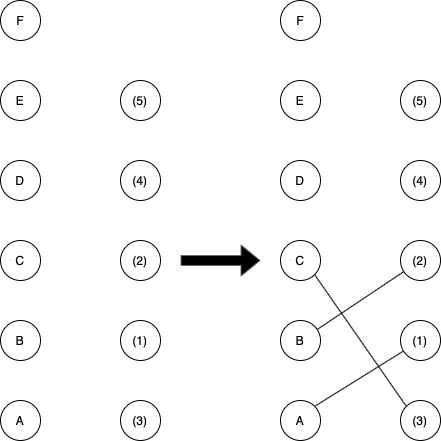
\includegraphics[width=0.5\linewidth]{{fig/fig_1.png}}
    \caption{Labelled $G$ and its trace after first $3$ iterations}
    \label{fig:1}
\end{figure}

As a rule of this \ilc{BFS}, the algorithm will try to match the node with lowest alphabetical value in $U$ to the node with lowest numerical value in $V$. Thus, the algorithm will check on edges $<A, (1)>$, $<B, (2)>$, and $C, (3)$ respectively. Since all of them are single edge argumenting pathes, we add all of them to $M$.

After these iterations, we achieved a matching $M$ which is identical to the maximal matching provided in problem. Thus, through emulation, we have proven the \textsc{Hopcroft-Karp} algorithm is capable of producing the given matching.

\section{Problem 2}

This problem will inherit the labelling, \ilc{BFS} rule, and list $M$ introduced by the above problem.

For $D, E, F \in U$, all of their conncted nodes $\in V$ are not free. Thus, stipulated by the \textsc{Hopcroft-Karp} algorithm, we will check for the free nodes $\in U$ for non-single-edged \textit{argumenting paths}.\newline

\begin{figure}[H]
    \centering
    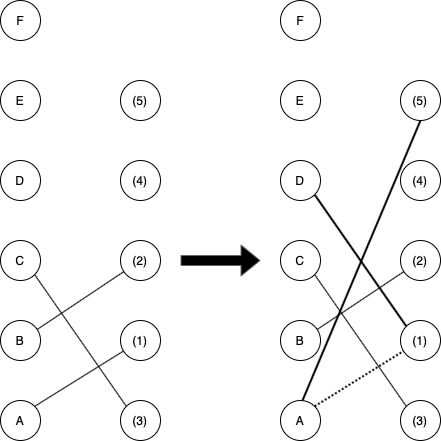
\includegraphics[width=0.5\linewidth]{{fig/fig_2.png}}
    \caption{Obtaining a maximum matching of $G$ from a given maximal matching}
    \label{fig:1}
\end{figure}

Starting with node $D$, as it has the lowerest alphabetical value of all free nodes $\in U$. It has two child nodes $\in V$, $\{(3), (1)\}$. We first check node $(1)$ as it has a lower numerical value. Since we are looking for an \textit{argumenting paths}, the only node we can proceed from $(1)$ is $A$, as it is the only \textit{matching node} (a node $\in M$) connected to $(1)$. Then, the only node we can proceed from $A$ is $(5)$, as it is the only free node conncted to $A$.

Now, we do a \ilc{DFS} from $(5)$ to $D$, we have discovered an \textit{argumenting paths} of $<D, (1), A, (5)>$. Thus, we remove the \textit{matching edge} $<A, (1)>$ from $M$, then add edge $<D, (1)>$ and $<A, (5)>$ to $M$.\newline

Since there will be no more \textit{argumenting paths} in the graph (as we can't find any more alternating path which starts and ends on free nodes). This $\{ <C, (3)>, <B, (2)>, <D, (1)>, <A, (5)> \}$ matching, with a cardinality of $4$, be the \textit{maximum matching} for the graph.

\section{Problem 3}

Imaging a subgraph $F$ of $G$, which is consisted by and only by edges in $M \sqcup N$ (edges that only $\in M$ or only $\in N$). Since $|M| > |N|$, we know that there must be $M \cap F > N \cap F$. Also for the ease of description, we initialize $M' = M$ and $N' = N$.

We also know that every node in $F$ will either have degree of $1$, where such node belongs and only belongs to $M$ or $N$; or degree of $2$, where such node is connected to an edge in $M$, and also conncted to an edge in $N$. \newline


We first inspect edges in $F$. If there is an edge $E \in M$ from $F$ that is a single edge (connected between two degree $1$ nodes), we remove it from $M'$ and add it to $N'$. This will make $|M'| = |M| - 1$ and $|N'| = N + 1$. We may tell that the new $M'$ and $N'$ are still matchings of $G$, due to the fact that for a single edge $\in M \sqcup N$, its two nodes are not connected to any edge of $M \cap N$, thus we won't have two edges of $N'$ sharing a node of $E$.\newline



If there is no single $E \in M$ from $F$, since $M \cap F > N \cap F$, there must be an alternating path $P$ in $F$ which starts and ends on edges of $M$. We inspect edges on this path: if an edge $EP \in P$ is also in $M$, we remove it from $M'$ and add it to $N'$; vice versa, if an edge $EP \in P$ is also in $N$, we remove it from $N'$ and add it to $M'$. Namely, we swapped the attribution of edges in $P$.

This maneuver will make $|M'| = |M| - 1$ and $|N'| = N + 1$, since path $P$ starts and ends on edges of $M$, there must be one more $M$ edge in $P$ than $N$ edges. Also the new $M'$ and $N'$ are still matchings of $G$, as the start- and end-nodes of path $P$ are not connecting to any edges from $M \cap N$.\newline


In both cases, we will have $M \cup N = M' \cup N'$ and $M \cap N = M' \cap N'$. Since we only swapped edge(s) in $M \sqcup N$ -- which won't effect the intersection and union of the two matchings.\newline





% \section{References}
%
% \nocite{*}
% \raggedright
% \bibliography{references.bib}
% \bibliographystyle{plain}


\end{document}